\section{Pipeline}
\label{autocorrelation:pipeline}

With all theory of preparatory work in place, the final method for modelling correlation structure can be detailed. 

The ensemble forecast, described in \cref{data}, is given as input to the marginal model, the feature model from \cref{basis}, giving estimated quantiles.

These quantiles are then interpolated into a full distribution using a monotone spline of 3. order, from \cref{distributions}.

The interpolated distribution is then used to transform the observed power production, \cref{data}, into pseudo-residuals, \cref{Pseudo}.

The pseudo-residuals are used to make a correlation corrected forecast using the \gls{sarma} model, found in \cref{autocorrelation},

Finally, the corrected forecast is translated back into the original space. Here to be evaluated using the methods in \cref{evaluation}

The whole process is illustrated in \cref{fig:autocorrelation:pipeline}.

\subsection{Modularity}

As was the intention of the original \gls{nabqr} method, the whole process is very modular\cite{jorgensenSequentialMethodsError2025}. Each part of the method can be changed without altering the other parts. 

For example, it is very possible that better model architectures can be found to estimate marginal quantiles.
This part of the model could then be changed while the rest is kept.

Likewise, a better way of interpolating/estimating the full distribution is possible, for example, using higher-order polynomials, which can then be implemented in the pipeline without changing anything else.

\begin{figure}[htb]
    \centering
    \caption[Correlation Pipeline]{Illustration of the correlation model pipeline.}
    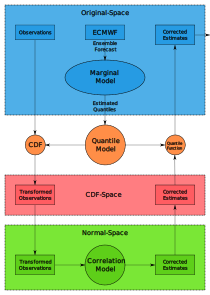
\includegraphics[width=1\linewidth]{Results/pipeline.pdf}
    \label{fig:autocorrelation:pipeline}
\end{figure}
